%======================================================================
% CAPITULO 3: GESTION DE CONEXIONES Y APLICACIONES
%======================================================================

\chapter{Gestion de Conexiones y Aplicaciones}
\label{ch:gestion}

\sdc{} permite gestionar multiples servidores y convertir servicios web en aplicaciones de escritorio independientes. Este capitulo detalla el proceso de configuracion de conexiones y despliegue de aplicaciones.

\section{Perfiles de Conexion}
\label{sec:conexiones}

El sistema permite gestionar multiples servidores remotos mediante perfiles de conexion configurables.

\begin{figure}[H]
\centering
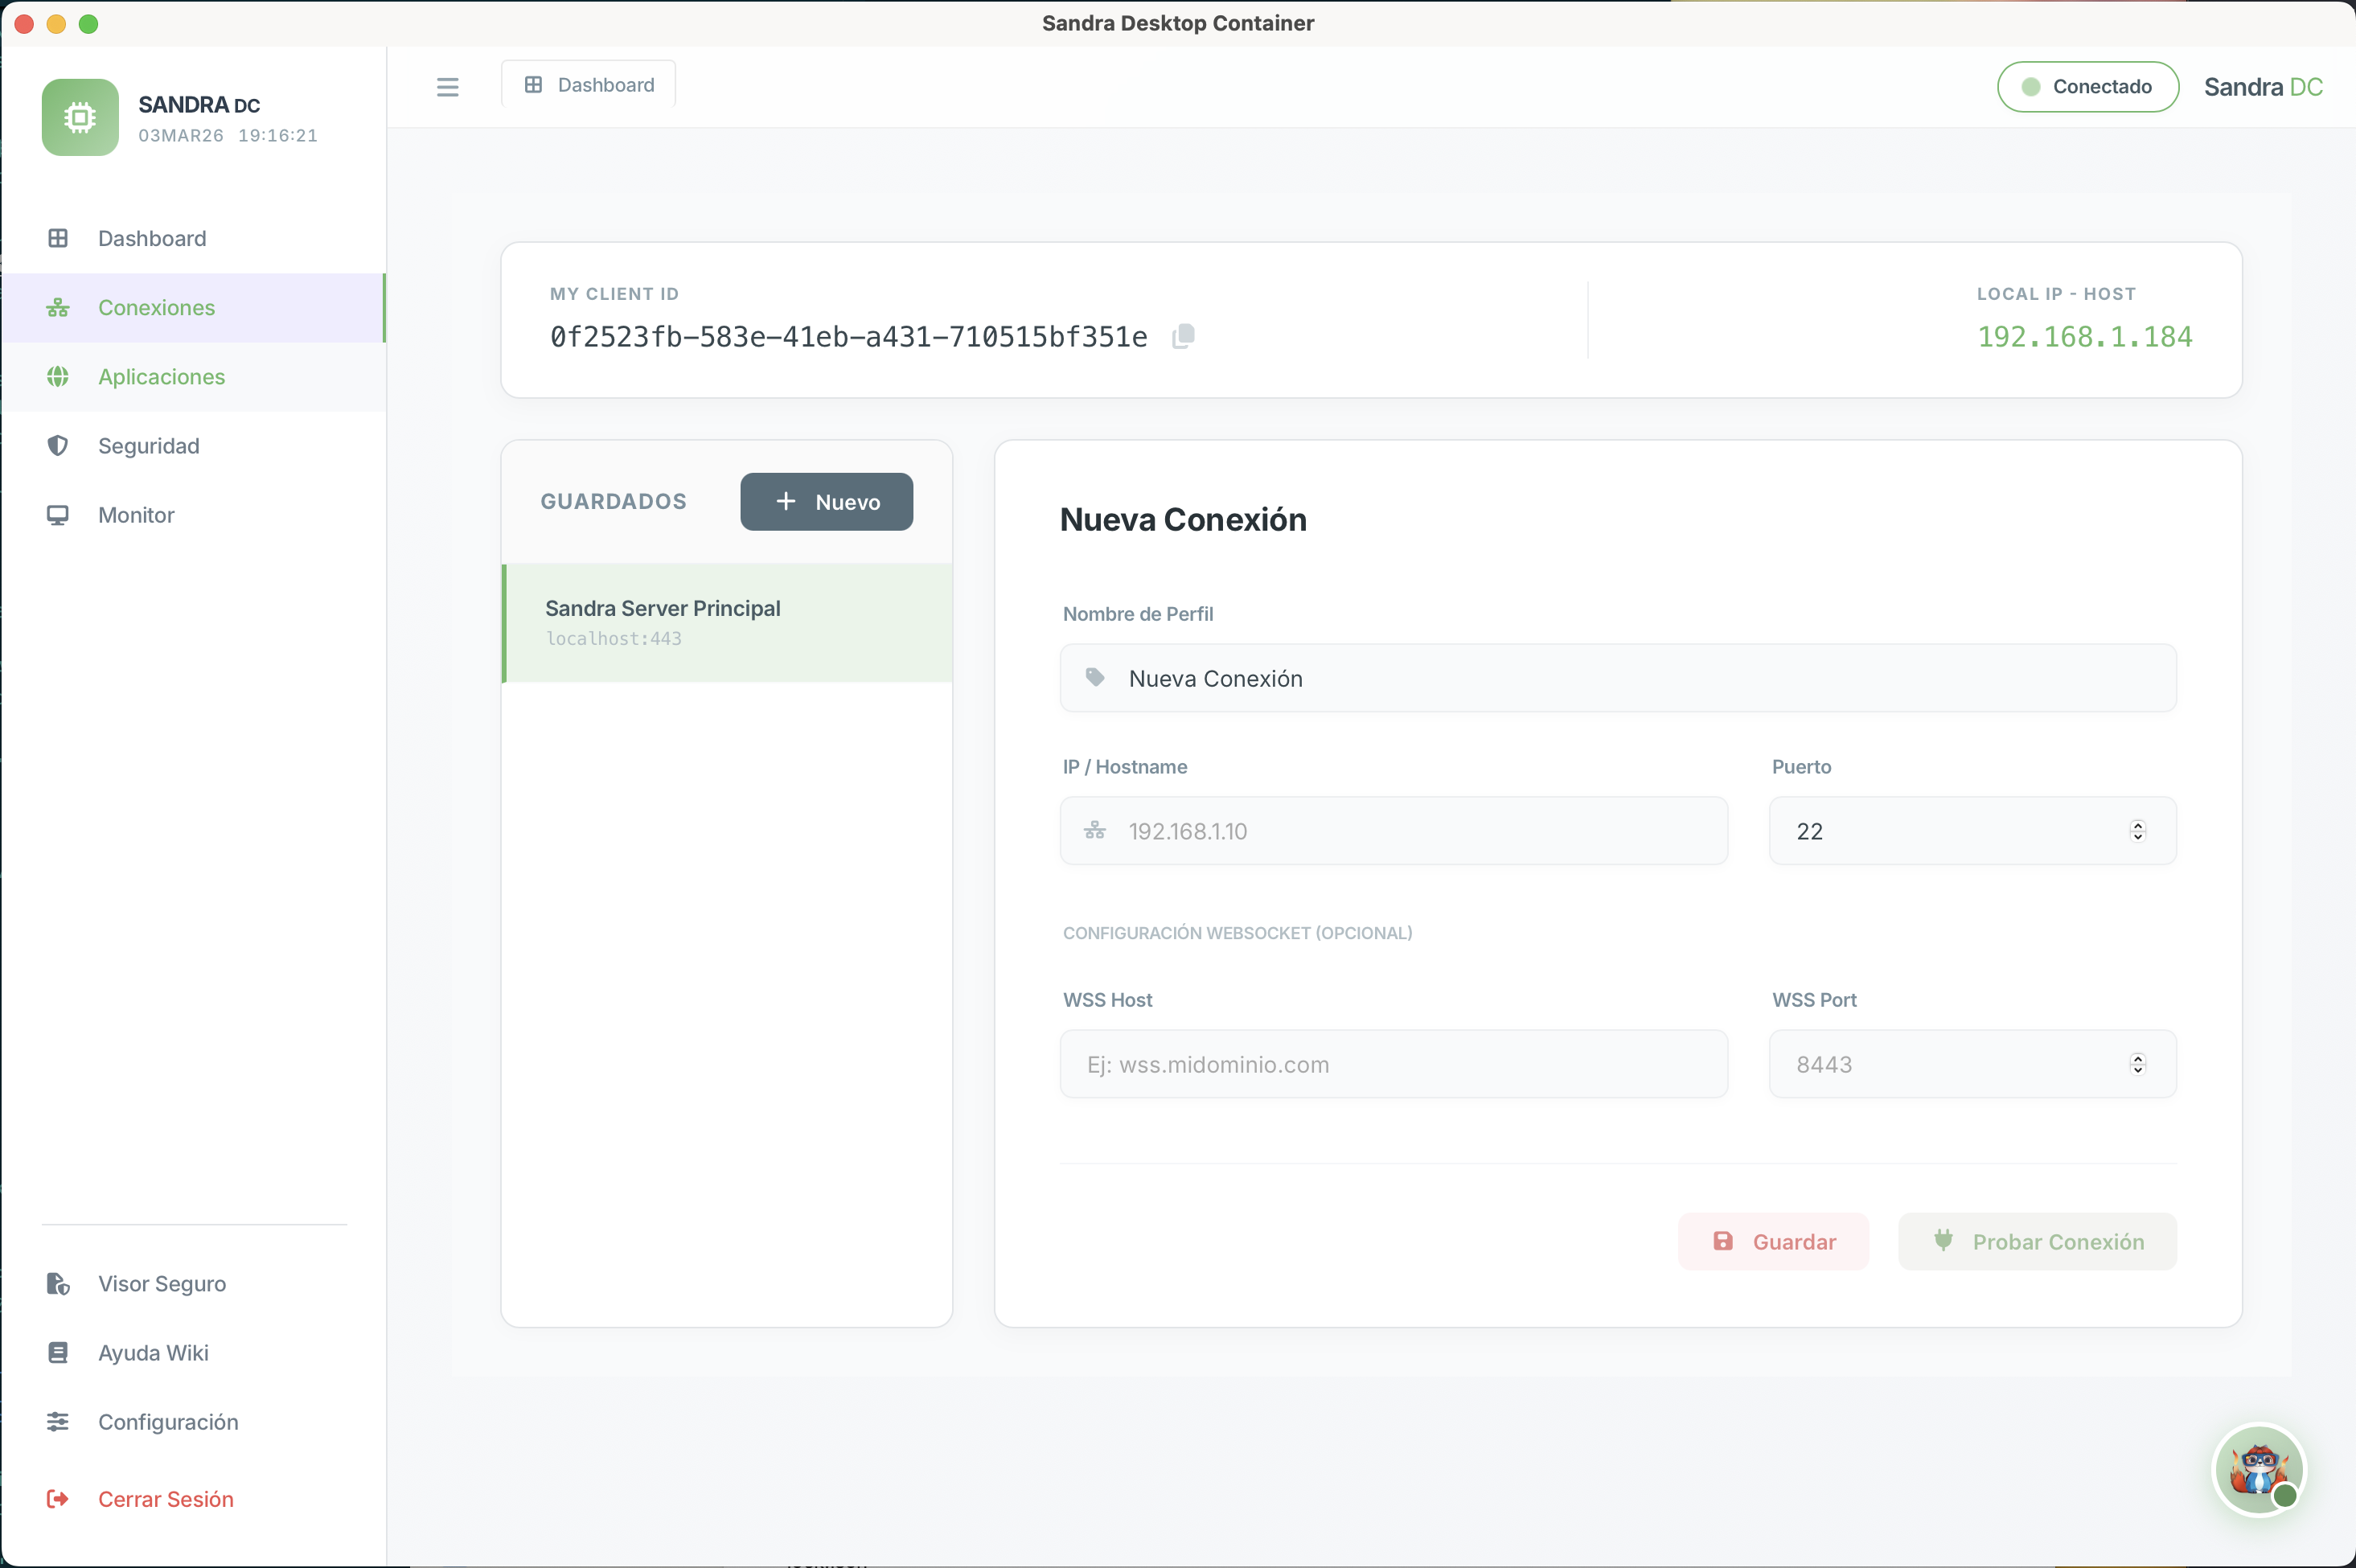
\includegraphics[width=0.95\textwidth]{anexos/5 conexion.png}
\caption{Interfaz de gestion de conexiones}
\label{fig:conexiones}
\end{figure}

\subsection{Creacion de Nueva Conexion}

Para establecer una nueva conexion a un servidor:

\begin{enumerate}[leftmargin=*]
    \item En el dashboard, hacer clic en Nueva Conexion
    \item Completar el formulario de configuracion basica
    \item Configurar opciones de seguridad (recomendado: WSS)
    \item Probar la conexion antes de guardar
    \item Asignar un nombre descriptivo al perfil
\end{enumerate}

\subsection{Parametros de Conexion}

\begin{table}[H]
\centering
\begin{tabular}{p{4cm}p{3cm}p{6cm}}
\toprule
\textbf{Parametro} & \textbf{Ejemplo} & \textbf{Descripcion} \\
\midrule
Host & servidor.com & Direccion IP o dominio \\
Puerto & 8443 & Puerto de escucha \\
Protocolo & WSS / WS & WebSocket Secure o WebSocket plano \\
Nombre & Produccion & Identificador del perfil \\
\bottomrule
\end{tabular}
\caption{Parametros de configuracion de conexion}
\label{tab:parametros-conexion}
\end{table}

\begin{quote}
\textbf{Seguridad de Conexiones}\\
Se recomienda utilizar siempre WSS (WebSocket Secure) en el puerto 8443 o superior. Las conexiones WS (sin cifrar) solo deben usarse en entornos de desarrollo controlados.
\end{quote}

\section{Despliegue de Aplicaciones}
\label{sec:aplicaciones}

Una de las caracteristicas distintivas de SDC es la capacidad de convertir servicios web en aplicaciones de escritorio independientes.

\begin{figure}[H]
\centering
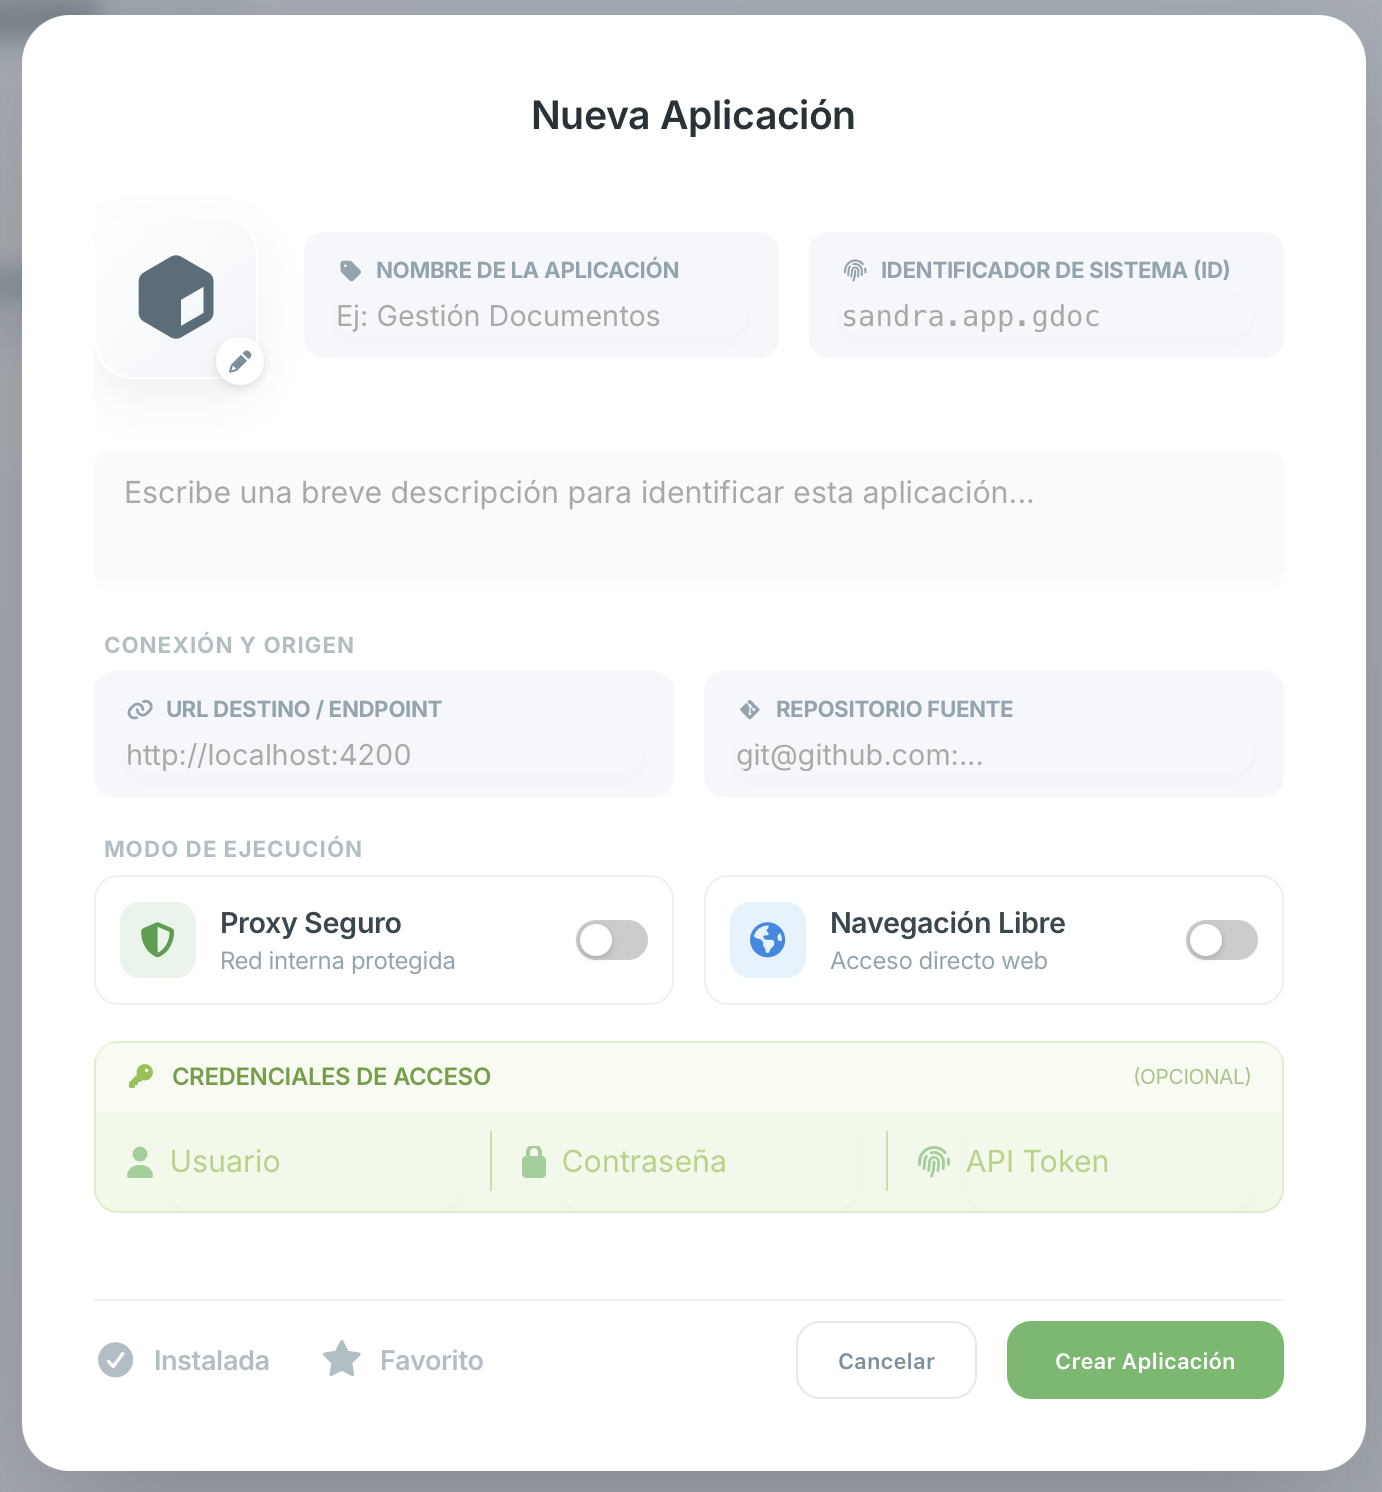
\includegraphics[width=0.95\textwidth]{anexos/6 aplicaciones.png}
\caption{Formulario de creacion de nueva aplicacion}
\label{fig:aplicaciones}
\end{figure}

\subsection{Modos de Despliegue}

\begin{table}[H]
\centering
\begin{tabular}{p{4cm}p{9cm}}
\toprule
\textbf{Modo} & \textbf{Descripcion} \\
\midrule
Proxy Seguro & Enmascara la IP real del contenedor mediante tuneles cifrados. Ideal para aplicaciones criticas. \\
\midrule
Navegacion Libre & Acceso directo sin tuneles de seguridad adicionales. Para aplicaciones internas de baja criticidad. \\
\bottomrule
\end{tabular}
\caption{Modos de despliegue de aplicaciones}
\label{tab:modos-despliegue}
\end{table}

\subsection{Repositorio Fuente}

SDC permite vincular aplicaciones a repositorios de codigo para habilitar despliegues automaticos:

\begin{lstlisting}[language=bash, caption={Configuracion de Repositorio}]
# Soporte para:
- GitHub (github.com/usuario/repo)
- GitLab (gitlab.com/usuario/repo)
- Bitbucket (bitbucket.org/usuario/repo)
- Repositorio privado (URL + credenciales)

# Opciones de despliegue automatico:
- Actualizar al iniciar
- Actualizar manualmente
- Actualizar programada (cron)
\end{lstlisting}

\begin{quote}
\textbf{Despliegue Automatico}\\
Cuando se activa el despliegue automatico, SDC verifica cambios en el repositorio cada 5 minutos y notifica al usuario cuando hay nueva version disponible.
\end{quote}

\section{Lista de Conexiones Activas}
\label{sec:conexiones-activas}

El panel de conexiones activas permite monitorear todas las conexiones establecidas.

\begin{figure}[H]
\centering
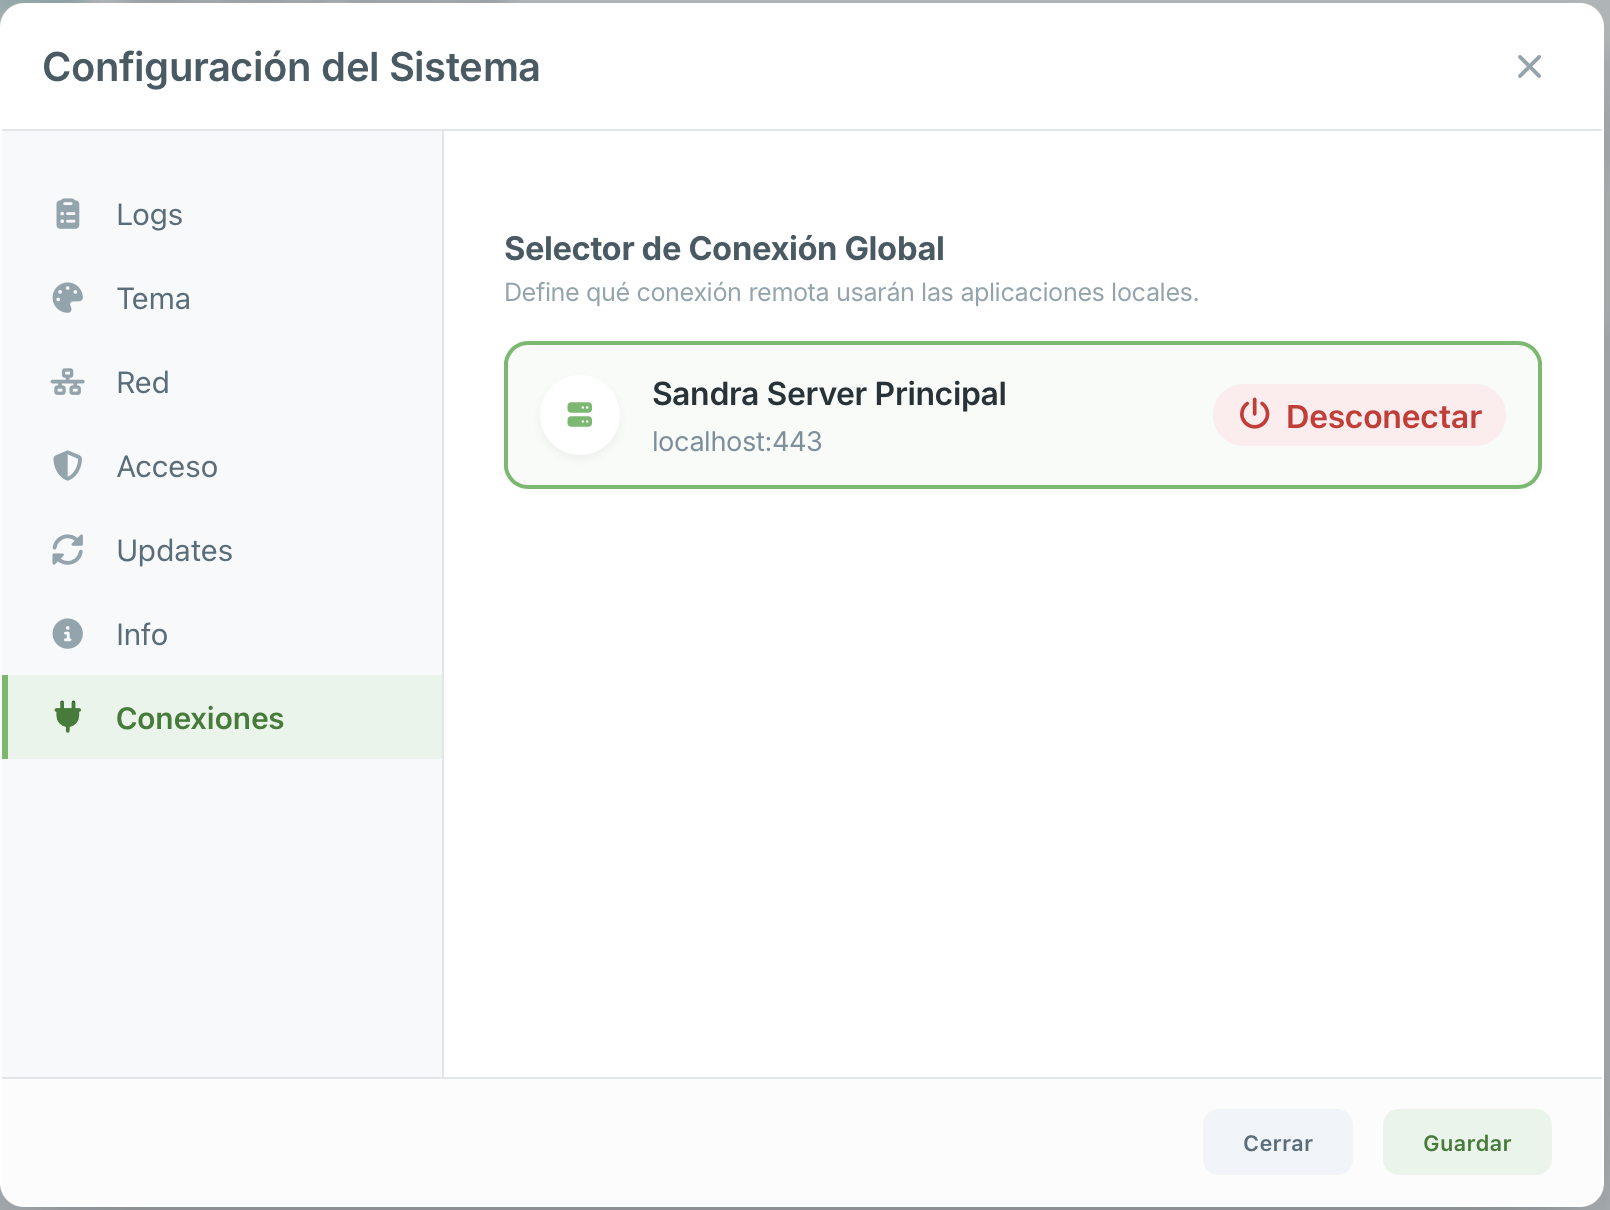
\includegraphics[width=0.95\textwidth]{anexos/16 conexiones activas.png}
\caption{Monitor de conexiones activas}
\label{fig:conexiones-activas}
\end{figure}

\subsection{Informacion Visualizada}

Para cada conexion activa, el sistema muestra:

\begin{itemize}[leftmargin=*]
    \item Estado (Verde: Activa, Rojo: Error, Gris: Inactiva)
    \item Nombre del perfil de conexion
    \item Host y puerto destino
    \item Tiempo de actividad (uptime)
    \item Latencia actual en ms
    \item Bytes transferidos
\end{itemize}

\section{Gestión del Monitor del Sistema}
\label{sec:monitor}

El modulo de monitoreo proporciona metricas detalladas de bajo nivel.

\begin{figure}[H]
\centering
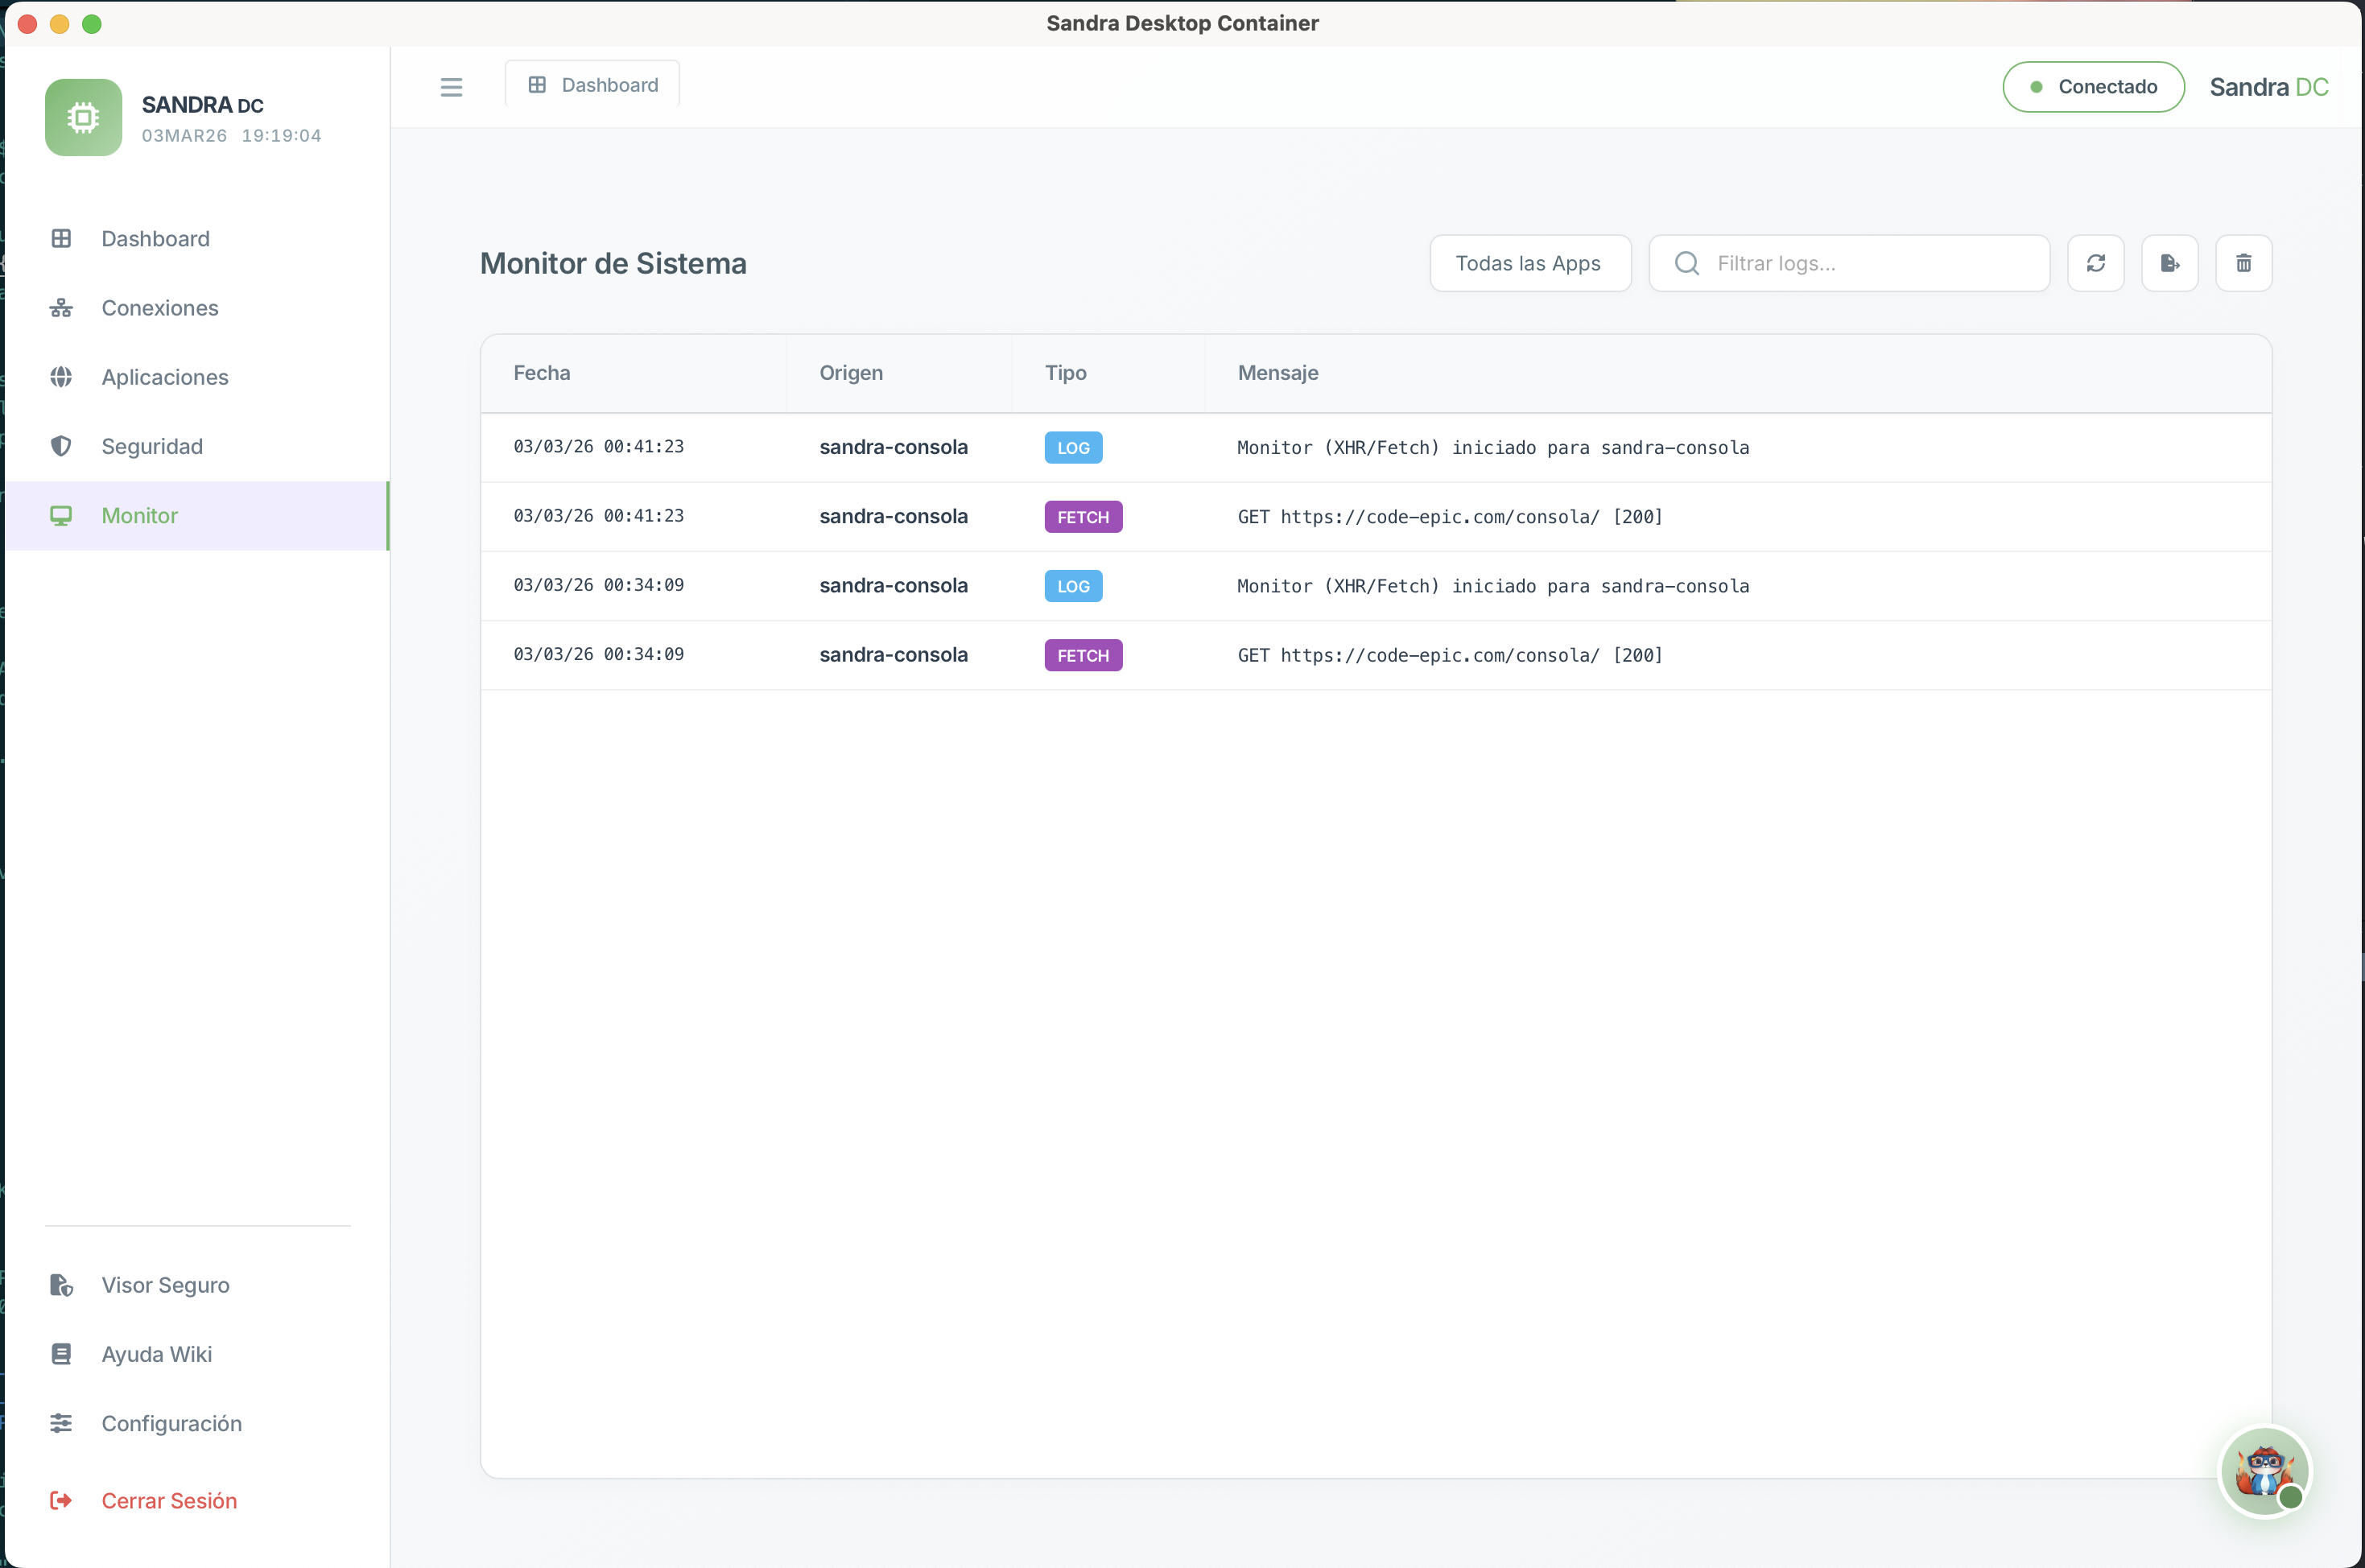
\includegraphics[width=0.95\textwidth]{anexos/10 monitor.png}
\caption{Monitor del sistema en tiempo real}
\label{fig:monitor}
\end{figure}

\subsection{Metricas de Hardware}

\begin{table}[H]
\centering
\begin{tabular}{p{3cm}p{5cm}p{5cm}}
\toprule
\textbf{Recurso} & \textbf{Metrica} & \textbf{Umbral de Alerta} \\
\midrule
CPU & Uso porcentual por nucleo & Mayor a 90 por ciento sostenido \\
RAM & Uso en GB / Total disponible & Mayor a 85 por ciento uso \\
Red & Paquetes/s y bytes/s & Latencia mayor a 500ms \\
Disco & I/O operaciones por segundo & Tiempo mayor a 100ms \\
\bottomrule
\end{tabular}
\caption{Metricas monitoreadas del sistema}
\label{tab:metricas-monitor}
\end{table}

\subsection{Inspector de Red}

Herramienta de transparencia que permite auditar el trafico de red:

\begin{itemize}[leftmargin=*]
    \item Interceptacion pasiva de peticiones Fetch/XHR
    \item Visualizacion de headers y payloads
    \item Filtrado por dominio, metodo HTTP o tipo de contenido
    \item Exportacion de logs para analisis forense
\end{itemize}

\begin{quote}
\textbf{Interceptacion Licita}\\
El Inspector de Red actua como herramienta de transparencia para auditores de seguridad. Su funcionamiento esta limitado al trafico generado por aplicaciones SDC.
\end{quote}
